%-------------------------------------------------------------------------------
% Fichero:	main.tex
% Documento:	Presentación para el taller "SODAR: Iniciación a Arduino + Processing"
% Este fichero almacena el cuerpo ppal de las transparencias.
% NO SE PUEDE COMPILAR directamente hay que usar el main.beamer.tex o el main.article.tex            
% Autores:	ctemes, eukelade, milo, salvari
% Fecha:        
% Descripción:	La presentación del taller
% Versión:      0.00
% Historial:    0.00 
%-------------------------------------------------------------------------------

% Quitamos el documentclass, lo vamos a poner a través de los ficheros
% main.beamer.tex  --> para hacer la presentación
% main.article.tex --> para hacer el artículo
% \documentclass{beamer}

\mode<presentation>
{
  \usetheme{Warsaw}
  \usecolortheme[RGB={52,170,205}]{structure}
  \setbeamertemplate{navigation symbols}{}
}
\usepackage{graphicx}
\DeclareGraphicsExtensions{.pdf,.png,.jpg} %solo para PDFLaTeX
\graphicspath{{figures/}{graphics/}{images/}}

% Esto es para poder escribir acentos directamente:
\usepackage[utf8]{inputenc}
% Esto es para que el LaTeX sepa que el texto está en español:
\usepackage[spanish]{babel}

% Links internos y externos
\usepackage{hyperref}

% Juegos de caracteres
\usepackage{bookman}
\usepackage{eurosym}

% \usepackage{times}
% \usepackage[T1]{fontenc}
% Or whatever. Note that the encoding and the font should match. If T1
% does not look nice, try deleting the line with the fontenc.

% Para listar código
\usepackage{color}
\definecolor{dkgreen}{rgb}{0,0.6,0}
\definecolor{gray}{rgb}{0.5,0.5,0.5}
\definecolor{mauve}{rgb}{0.58,0,0.82}

\usepackage{listings}

% Empezamos fijando el estilo para el código Arduino

\lstset{language=C++,
  basicstyle=\tiny\ttfamily,
  keywordstyle=\color{blue}\ttfamily,
  stringstyle=\color{red}\ttfamily,
  commentstyle=\color{green}\ttfamily,
  morecomment=[l][\color{magenta}]{\#}
}


\title[Taller SODAR] % (optional, use only with long paper titles)
{SODAR: Iniciación a Arduino + Processing}

\subtitle
{Un taller BricoLabs} % (optional)

\author[ctemes, eukelade, milo, salvari] % (optional, use only with lots of authors)
{ctemes \and eukelade \and Milo \and salvari}
% - Use the \inst{?} command only if the authors have different
%   affiliation.

\institute[BricoLabs] % (optional, but mostly needed)
{
Asociación BricoLabs 
}
% - Use the \inst command only if there are several affiliations.
% - Keep it simple, no one is interested in your street address.

\date[Short Occasion] % (optional)
{7 noviembre / OSHWDem - 2014}

\subject{Taller Arduino Processing}
% This is only inserted into the PDF information catalog. Can be left
% out. 



% If you have a file called "university-logo-filename.xxx", where xxx
% is a graphic format that can be processed by latex or pdflatex,
% resp., then you can add a logo as follows:

% \pgfdeclareimage[height=0.4cm]{oshwdem-logo}{oshwi.png}
% \logo{\pgfuseimage{oshwdem-logo}}
\logo{
\includegraphics [width=0.2\textwidth]{oshwi.png}}



% Delete this, if you do not want the table of contents to pop up at
% the beginning of each subsection:
\AtBeginSubsection[]
{
  \begin{frame}<beamer>{Agenda}
    \tableofcontents[currentsection,currentsubsection]
  \end{frame}
}


% If you wish to uncover everything in a step-wise fashion, uncomment
% the following command: 

%\beamerdefaultoverlayspecification{<+->}


\begin{document}

\begin{frame}
  \titlepage
\end{frame}

\begin{frame}{Agenda}
  \tableofcontents
  % You might wish to add the option [pausesections]
  \note[item]{Recordar que el curso es de iniciación}
  \note[item]{Va a ser un curso intenso, descanso cortito}
  \note[item]{Comentar duración total del curso}
\end{frame}


%______________________________________________________________________
\section{Presentación}

%......................................................................
\subsection{¿Quienes somos?}

%----------------------------------------------------------------------
\begin{frame}{BricoLabs y la OSHWDem}
  \begin{columns}
    \column{.6\textwidth}
    
\includegraphics [width=0.8\textwidth]{bricolabs_logo.png}

    \url{http://bricolabs.cc/}

    \column{.4\textwidth}
    
\includegraphics [width=0.8\textwidth]{oshwi.png}

    \url{http://oshwdem.org}
  \end{columns}
  \note[item]{BricoLabs: Asociación, Domus, Difusión del hardware y
    software libre, Tecnófilos, Divulgación, wiki, }
  \note[item]{OSHWDem evento barcamp}
\end{frame}

%----------------------------------------------------------------------
\begin{frame}{Ponentes}
  \begin{itemize}
  \item @ctemes
  \item Eukelade @pepdiz
  \item Milo
  \item @salvari
  \end{itemize}
  \note[item]{Para cualquier duda podéis contactar con nosotros en
    nuestros twitters}
\end{frame}

%----------------------------------------------------------------------
\begin{frame}{Asistentes}
  \begin{itemize}
  \item ¿Quién conoce el Arduino?
    \pause
  \item ¿Quién conoce Processing?
    \pause
  \item ¿Traéis los deberes hechos? ;)
  \end{itemize}
  \note[item]{No hay mucho más que añadir}
\end{frame}

%......................................................................
\subsection{Requisitos}

%----------------------------------------------------------------------
\begin{frame}{Revisar la instalación}
  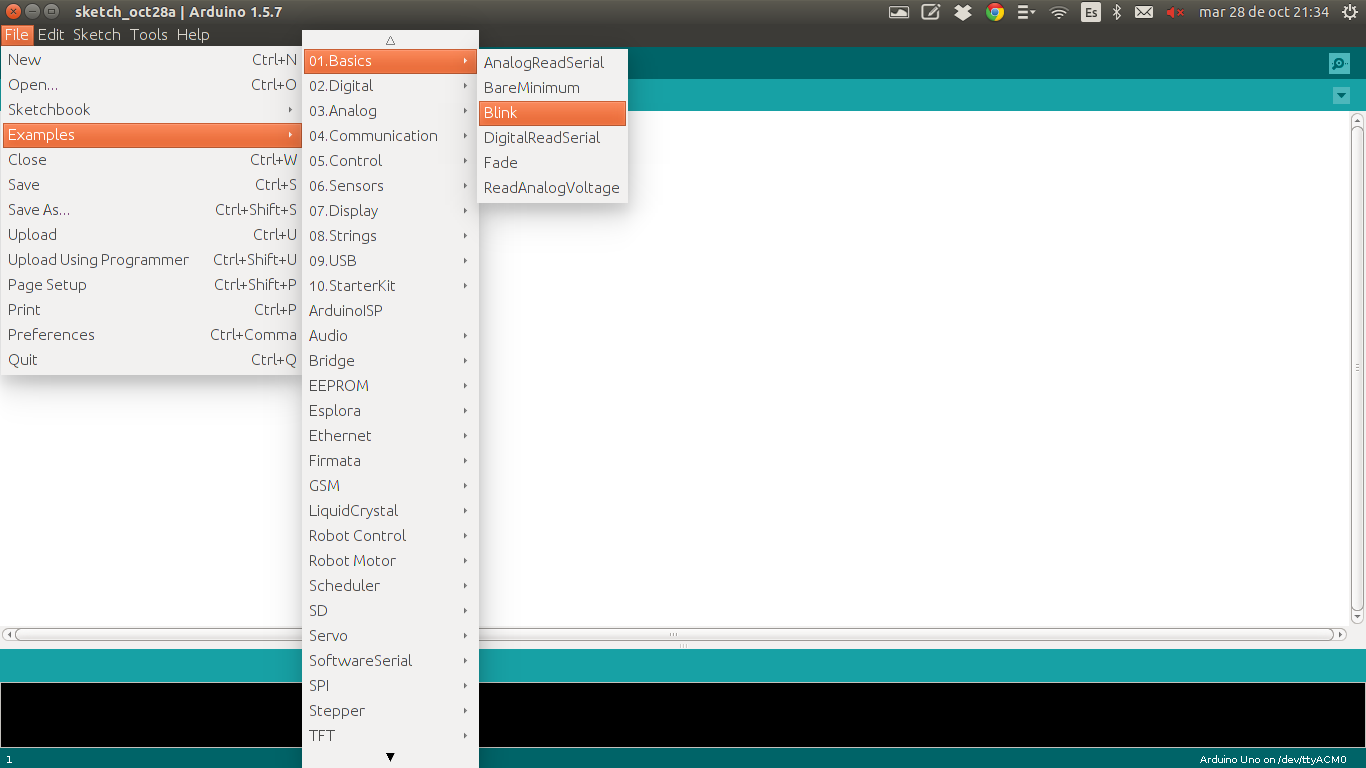
\includegraphics [width=0.8\textwidth]{open_blink.png}
  \note[item]{Separamos a los que tienen hecha la instalación y los
    que no, los primeros prueban el Blink y a los segundos los
    ayudamos.}
  \note[item]{Hora límite 17.00}
  \note[item]{Blink: Fichero::Ejemplos::Básicos::Blink}
\end{frame}

%______________________________________________________________________
\section{Arduino}

%......................................................................
\subsection{Intro}

%----------------------------------------------------------------------
\begin{frame}{SODAR}

  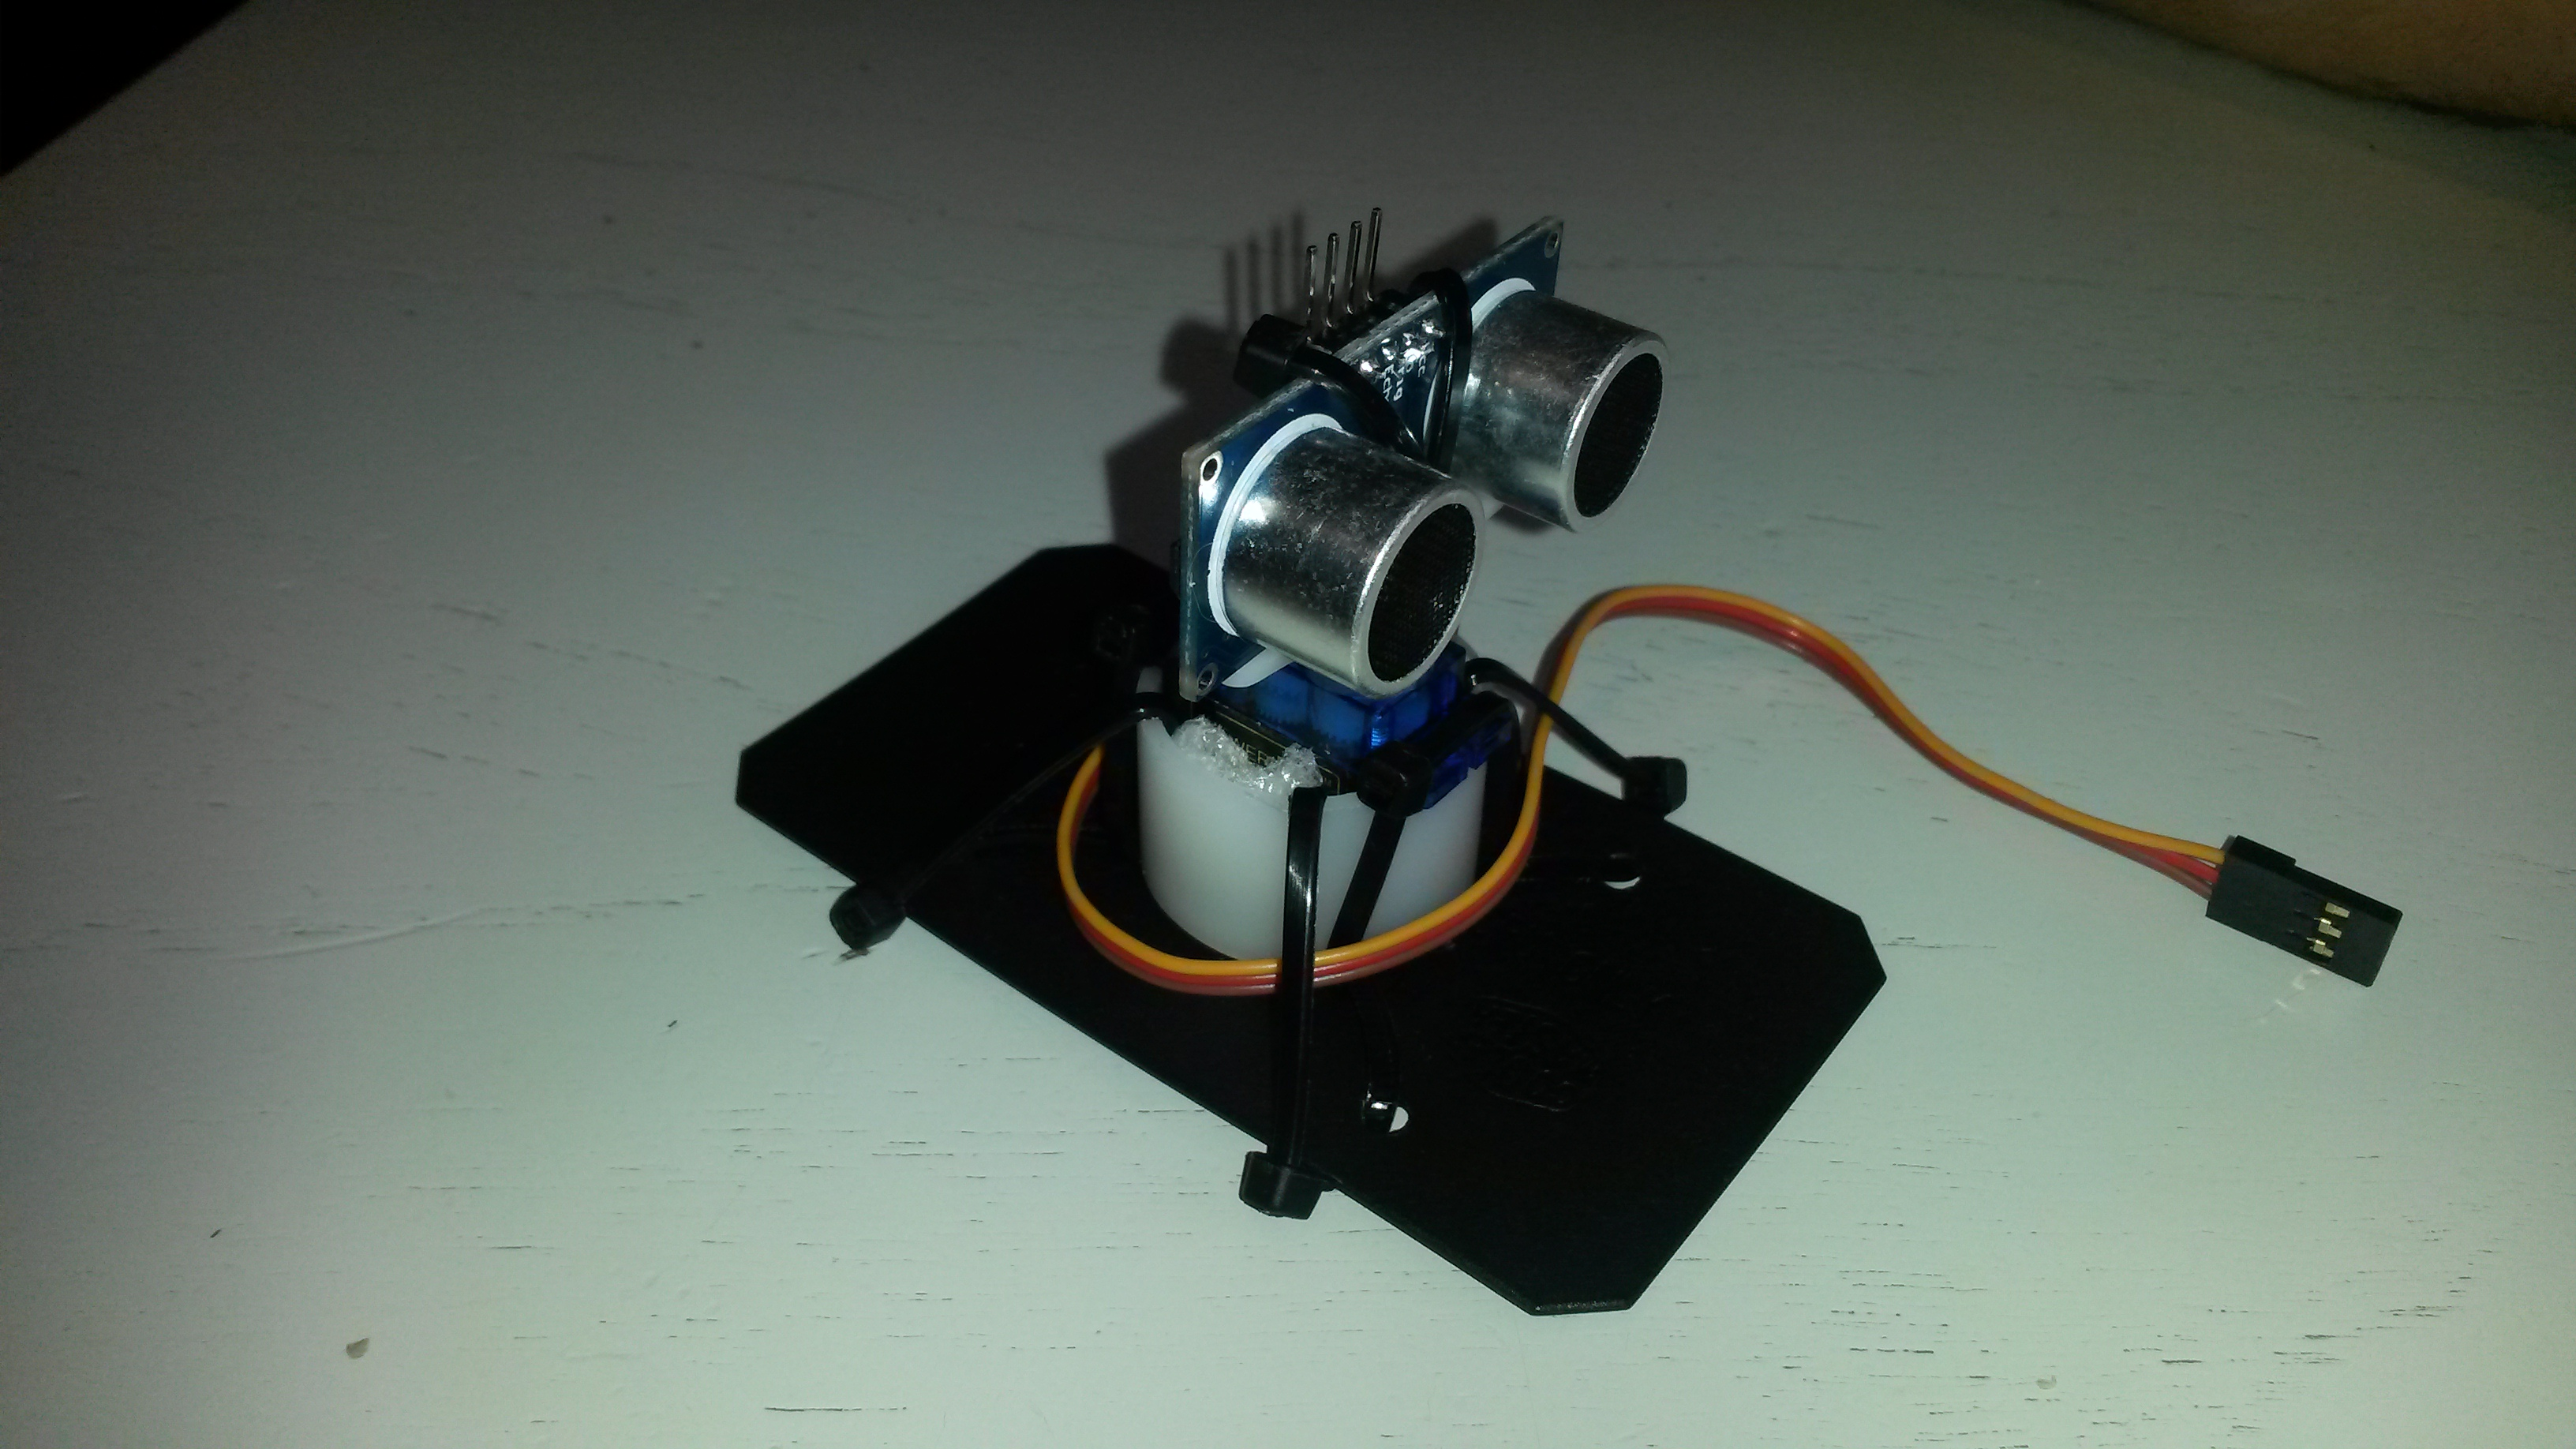
\includegraphics [width=0.8\textwidth]{montaje.jpg}

  \note[item]{SODAR, igual que RADAR SOnic Detection and Range}
  \note[item]{Básicamente dos partes moviento y sensor}
  \note[item]{Una tercera parte será la estación de usuario}
\end{frame}

%----------------------------------------------------------------------
\begin{frame}{Arduino}

  \begin{figure}
    \centering
    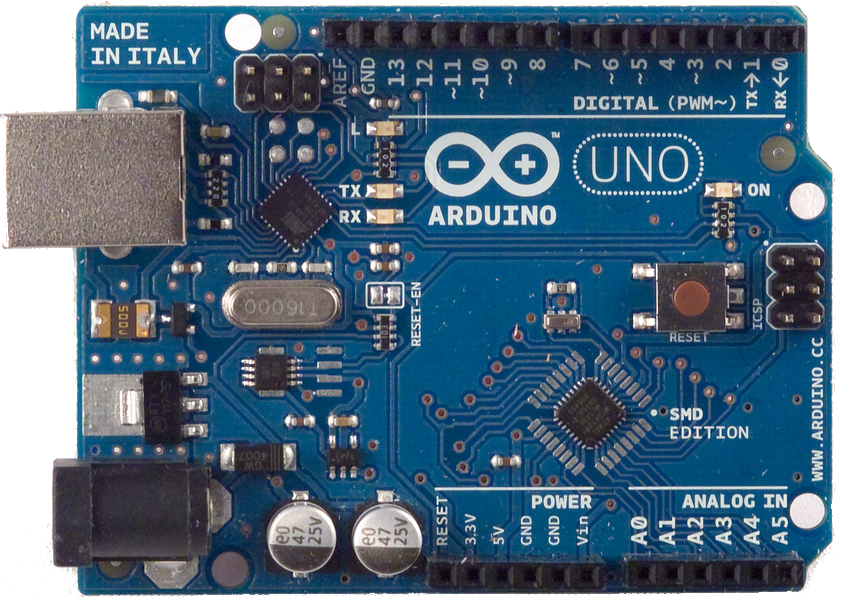
\includegraphics [width=0.7\textwidth]{ArduinoUnoSmd.jpg}
  \end{figure}
  \begin{columns}
    \column{.5\textwidth}
    \href{http://www.arduino.cc/}{Página Principal}
    \column{.5\textwidth}
    \href{http://blog.arduino.cc/wp-content/uploads/2013/11/ArduinoEvolution_make.jpg}{Foto Familia}
  \end{columns}
  \note[item]{Empezamos con el Arduino}
  \note[item]{Año 2005}
  \note[item]{Procesadores de la familia Atmel AVR (AtMega)}
  \note[item]{IDE (basado en processing)}
  \note[item]{CPP con librerias variadas}
\end{frame}

%......................................................................
\subsection{Montaje}

%----------------------------------------------------------------------
\begin{frame}{Montaje I}
  Foto del soporte
\end{frame}

%----------------------------------------------------------------------
\begin{frame}{Montaje II}
  Esquema Fritzing
  \note[item]{¡Mucho ojo con los cables del servo!}
  \note[item]{Rojo: 5 volt}
  \note[item]{Marron: tierra}
  \note[item]{Naranja: Señal}
\end{frame}

%......................................................................
\subsection{Movimiento}

%----------------------------------------------------------------------
\begin{frame}[fragile]{Estructura de un programa Arduino}
\begin{lstlisting}
#include <Servo.h>     

#define SERVO_PWM_PIN 9

Servo myservo;         

/*----------------------------------------------------------------------
  setup
   Se ejecuta una sola vez al principio del programa. O cuando el arduino
   se resetea.
 ----------------------------------------------------------------------*/
void setup() {
  
}

/*----------------------------------------------------------------------
  loop
   Se ejecuta siempre, hasta el fin de los tiempos :-)
 ----------------------------------------------------------------------*/
void loop() {

}
\end{lstlisting}
\note[item]{Tres partes}
\note[item]{Primera parte imports y variables -- Tiempo de compilación}
\note[item]{Tiempo de ejecución -- dos partes setup y loop}
\note[item]{setup al arrancar, después de un reset hay un arranque}
\note[item]{loop para siempre jamás (mentira)}
\end{frame}

%----------------------------------------------------------------------
\begin{frame}{Servo}
  Foto del servo

  Fundido a Código de Invocación del servo

  \note[item]{Que es un servo? Un motor y un pequeño circuito}
  \note[item]{Protocolo de comunicación, anterior a la era digital}
  \note[item]{PWM: 20ms de periodo para los servos}
  \note[item]{Tipos de servos, los nuestros son de 180 grados, 1,6 kg}
  
\end{frame}

%----------------------------------------------------------------------
\begin{frame}{Barridos}
  Foto de un radar (de verdad)

  \note[item]{¿Como os imagináis que debe moverse el radar?}
\end{frame}

%----------------------------------------------------------------------
\begin{frame}{Una solución}
  Nuestra solución \note[item]{Vemos nuestra solución en el IDE
    proyectado y comentamos}
\end{frame}

%......................................................................
\subsection{Sensor}

%----------------------------------------------------------------------
\begin{frame}{Sensor ultrasonidos}
  Foto sensor

  Fundido a Caracteristicas técnicas

  \note[item]{Como funciona el sensor, tren de pulsos y mide el tiempo
    en que tarda en recibir el eco}
\end{frame}

%----------------------------------------------------------------------
\begin{frame}{Protocolo}
  Diagrama de señales

  \note[item]{Explicamos el protocolo de señales del servo}
\end{frame}

% \definecolor{dkgreen}{rgb}{0,0.6,0}
% \definecolor{gray}{rgb}{0.5,0.5,0.5}
% \definecolor{mauve}{rgb}{0.58,0,0.82}
% 
% \lstset{frame=tb,
%   language=Java,
%   aboveskip=3mm,
%   belowskip=3mm,
%   showstringspaces=false,
%   columns=flexible,
%   basicstyle={\small\ttfamily},
%   numbers=none,
%   numberstyle=\tiny\color{gray},
%   keywordstyle=\color{blue},
%   commentstyle=\color{dkgreen},
%   stringstyle=\color{mauve},
%   breaklines=true,
%   breakatwhitespace=true,    // added this
%   tabsize=3
% }

\end{document}


